% !TEX program = xelatex -shell-escape
% !TEX spellcheck = cs_CZ

% Nejprve uvedeme tridu dokumentu s volbami
\documentclass[czech,master]{diploma}
% Dalsi doplnujici baliky maker
\usepackage[autostyle=true,czech=quotes]{csquotes} % korektni sazba uvozovek, podpora pro balik biblatex
\usepackage[backend=biber, style=iso-numeric, alldates=iso]{biblatex} % bibliografie

\usepackage{dcolumn} % sloupce tabulky s ciselnymi hodnotami
\usepackage{subfig} % makra pro "podobrazky" a "podtabulky"
\usepackage{xevlna}
\usepackage{tikz}
\usepackage{mathtools}
\usepackage{amsmath}
\usepackage{amssymb}
\usepackage{bm}
\usepackage{esvect}
\usepackage{pgfplots}
\usepackage{fontspec}
\usepackage{minted}
\usepackage[autostyle=true,czech=quotes]{csquotes} % korektni sazba uvozovek, podpora pro balik biblatex
\usepackage{pifont}
\usepackage{xcolor}
\usepackage{hyperref}

%\setmonofont{[JetBrainsMono-Regular.ttf]}[Contextuals=Alternate,Ligatures=TeX]
%\setmonofont{[Computer Modern]}

\renewcommand{\listingscaption}{Výpis}

\pdfminorversion=6

%Značení normovaného vektoru
%\newcommand{\uvec}[1]{\boldsymbol{\hat{#1}}}

\newcommand{\interval}[1]{\left[{#1}\right]}
\newcommand{\uvec}[1]{\hat{#1}}

\newcommand{\point}{p}

\newcommand{\brdf}{f_r\left(\point,\omega_{o},\omega_{i}\right)}
\newcommand{\normVec}{\uvec{n}}
\newcommand{\inVec}{\omega_{i}}
\newcommand{\outVec}{\omega_{o}}
\newcommand{\refl}{\omega_{r}}
\newcommand{\halfVec}{\uvec{h}}

\newcommand{\outRadiance}{L_o\left(\point,\outVec\right)}
\newcommand{\inRadiance}{L_i\left(\point,\inVec\right)}
\newcommand{\emitRadiance}{L_e\left(\point\right)}
\newcommand{\irradiance}{E\left(\point,\inVec\right)}


\newcommand{\inDotNorm}{\left(\inVec\cdot\normVec\right)}

\newcommand{\randU}{\xi_{1}}
\newcommand{\randV}{\xi_{2}}

\newcommand{\alb}{\rho}
\newcommand{\rough}{\sigma}
\newcommand{\ior}{f_0}

\newcommand{\fromVect}{f}
\newcommand{\toVect}{t}

\pgfplotsset{compat=newest}


\newminted{c++}{
    style=vs,
    frame=lines
}


\newcommand{\true}{\ding{51}}
\newcommand{\false}{\ding{55}}
\newcommand{\undecided}{\dots}

% Zadame pozadovane vstupy pro generovani titulnich stran.
\ThesisAuthor{Richard Zvonek}

\ThesisSupervisor{Ing. Tomáš Fabián, Ph.D.}

\CzechThesisTitle{Interaktivní prohlížeč BRDF funkcí}

\EnglishThesisTitle{Interactive Visualization of BRDF Functions}

\SubmissionYear{2021}

% Pokud nechceme nikomu dekovat makro zapoznamkujeme.
% \Acknowledgement{Rád bych na tomto místě poděkoval všem, kteří mi s prací pomohli, protože bez nich by tato práce nevznikla.}

\CzechAbstract{TODO Czech abstract}

\CzechKeywords{TODO Klíčová slova}

\EnglishAbstract{TODO Eng abstract}

\EnglishKeywords{TODO keywords}

\AddAcronym{BRDF}{bidirectional reflectance distribution function}
\AddAcronym{IOR}{index of refraction}
\AddAcronym{PDF}{probability density function}

\addbibresource{main.bib}

% Novy druh tabulkoveho sloupce, ve kterem jsou cisla zarovnana podle desetinne carky
\newcolumntype{d}[1]{D{,}{,}{#1}}


% Zacatek dokumentu
\begin{document}

% Nechame vysazet titulni strany.
\MakeTitlePages
% A nasleduje text zaverecne prace.

\chapter{Úvod}
TODO


\clearpage
\chapter{Užité symboly}
Z důvodu použití vyššího množství matematických symbolů v této diplomové práci jsem sjednotil značení použité ve vzorcích. Přehled těchto vzorců s případným doplněním detailů je uveden v následujícím seznamu.
\section{Obecné}
\begin{itemize}
  \item[\(\outRadiance\):] Výsledná zář vyzařovaná z daného bodu
  \item[\(\emitRadiance\):] Zář, pasivně vyzařovaná z objektu v daném bodě
  \item[\(\inRadiance\):] Zář dopadající na daný bod
  \item[\(\irradiance\):] Celková žář dopadající na daný bod
  \item[\(\brdf\):] BRDF funkce
  \item[\(\left(\theta,\phi\right)\):] Vektor definovaný sférickými souřadnicemi
  \item[\(\left(x,y,z\right)\):] Vektor definovaný kartézskými souřadnicemi
  \item[\(\normVec\):] Vektor normály povrchu
  \item[\(\inVec\):] Vektor ve směru ke světelnému zdroji. Platí: \(\inVec = \left(\theta_i,\phi_i\right)\)
  \item[\(\outVec\):] Vektor ve směru k pozorovateli. Platí: \(\outVec = \left(\theta_o,\phi_o\right)\)
  \item[\(\refl\):] Vektor zrcadlového odrazu světla, platí: \(\refl = 2\left(\inVec\cdot\normVec\right)\normVec-\inVec\)
  \item[\(\halfVec\):] Poloviční vektor mezi pohledovým a světelným vektorem. Platí: \(\halfVec = \frac{\inVec + \outVec}{\| \inVec + \outVec\|}\)
  \item[\(\theta_r\):] Úhel odrazu, platí: \(\cos\theta_r = \outVec\cdot\refl\)
\end{itemize}

\section{Vzorkování}

\begin{itemize}
  \item[\(\randU\):] Náhodné číslo \(\in \mathbb{R}, \interval{0,1}\)
  \item[\(\randV\):] Náhodné číslo \(\in \mathbb{R}, \interval{0,1}\)
\end{itemize}

\section{BRDF}

\begin{itemize}
  \item[\(\alb\):] Albedo materiálu, poměr mezi pohlceným a odraženým světlem (Lambert)
  \item[\(k_s\):] Koeficient odrazivosti materiálu (Phong)
  \item[\(k_d\):] Koeficient difuze materiálu (Phong)
  \item[\(n\):] Koeficient lesklosti materiálu (Phong)
  \item[\(\rough\):] Koeficient drsnosti povrchu --- roughness (Torrance-Sparrow, Cook-Torrance, Oren-Nayar)
  \item[\(\ior\):] Koeficient lomu světla --- ior (Torrance-Sparrow, Cook-Torrance)
\end{itemize}

\clearpage
\chapter{Fotorealistický rendering}
Počítačová grafika se odjakživa snaží svými výsledky co nejvěrněji přiblížit reálnému světu. Fotorealistická grafika je taková, která se tváří jako nerozeznatelná např.\ od fotografie. Pro fotorealismus je nutné, aby rendering (výpočet geometrie, pozice objektů a osvětlení) co nejpřesněji simuloval fyzikální principy šíření světla. V roce 1986 byl realistický rendering popsán integrální rovnicí popisující přenos světelné energie ve scéně. Renderovací rovnice byla popsána simultánně ve článcích~\cite{KajiyaRenderEq} a~\cite{ImmelRenderEq}. Kajiya v~\cite{KajiyaRenderEq} popisuje různé možnosti řešení integrálu renderovací rovnice, mimo jiné i pomocí Monte Carlo metody, kterou pojmenoval jako path tracing~\cite{HainesRayTracingGems2019}. Immel, Cohen a Greenberg v článku~\cite{ImmelRenderEq} navrhují řešení renderovací rovnice pomocí metody konečných prvků, kterou pojmenovali jako metodu radiozity. V této práci se budu dále zabývat řešením renderovací rovnice pouze pomocí metody Monte Carlo. \par
Renderovací rovnici lze vyjádřit \hyperref[eq:render]{vzorcem~\ref{eq:render}}. Renderovací rovnice bez BRDF členu a bez emisivního členu vyjadřuje intenzitu záření dopadající na danou plochu (viz \hyperref[eq:renderIrradiance]{vzorec~\ref{eq:renderIrradiance}})\cite{Dutre2003GICompendum}.

\begin{equation} \label{eq:render}
  \outRadiance = \emitRadiance + \int_{H \left( \point \right)}^{~}\inRadiance \brdf \inDotNorm \,d\inVec
\end{equation}

\begin{equation} \label{eq:renderIrradiance}
  \emitRadiance = \int_{H \left( \point \right)}^{~}\inRadiance \inDotNorm \,d\inVec
\end{equation}

\section{Osvětlení}
Jak už bylo zmíněno, realistický rendering se zabývá co nejpřesnější simulací šíření světla ve scéně. V reálném světě je světlo jako takové elektromagnetické záření. Viditelná část světla odpovídá zhruba intervalu \(\interval{390;760}nm\) vlnové délky. Při renderingu se často pracuje pouze s geometrickou optikou. Geometrická optika zjednodučuje při šíření světla světelné paprsky na pouhé vektory, zanedbává vlastnosti vycházející z vlnové podstaty světla. Z pohledu počítačové simulace jsou světelné paprsky vyzařovány světelnými zdroji do scény. Objekty ve scéně světelné paprsky pohlcují a nebo odráží. Odraz a pohlcení světla potom definuje, jak výsledný objekt působí. \par
Osvětlení objektů ve scéně je popsáno osvětlovacím modelem. Pokud daný osvětlovací model bere v potaz vliv na osvětlení pouze přímými zdroji světla, jedná se o lokální osvětlovací model. Pokud osvětlovací model bere v potaz i světlo odražené ostatními objekty ve scéně, které samy o sobě žádné světlo nevyzařují, jedná se o globální osvětlovací model. Rozdíl mezi osvětlením lokálním a globálním osvětlovacím modelem je patrný z \hyperref[fig:localVsGlobalIllum]{obrázku~\ref{fig:localVsGlobalIllum}}\footnote{Výsledné renderované obrázky byly vytvořeny v programu Blender 2.92}.

\begin{figure}[ht]%
  \centering
  \subfloat[Lokální osvětlovací model]{{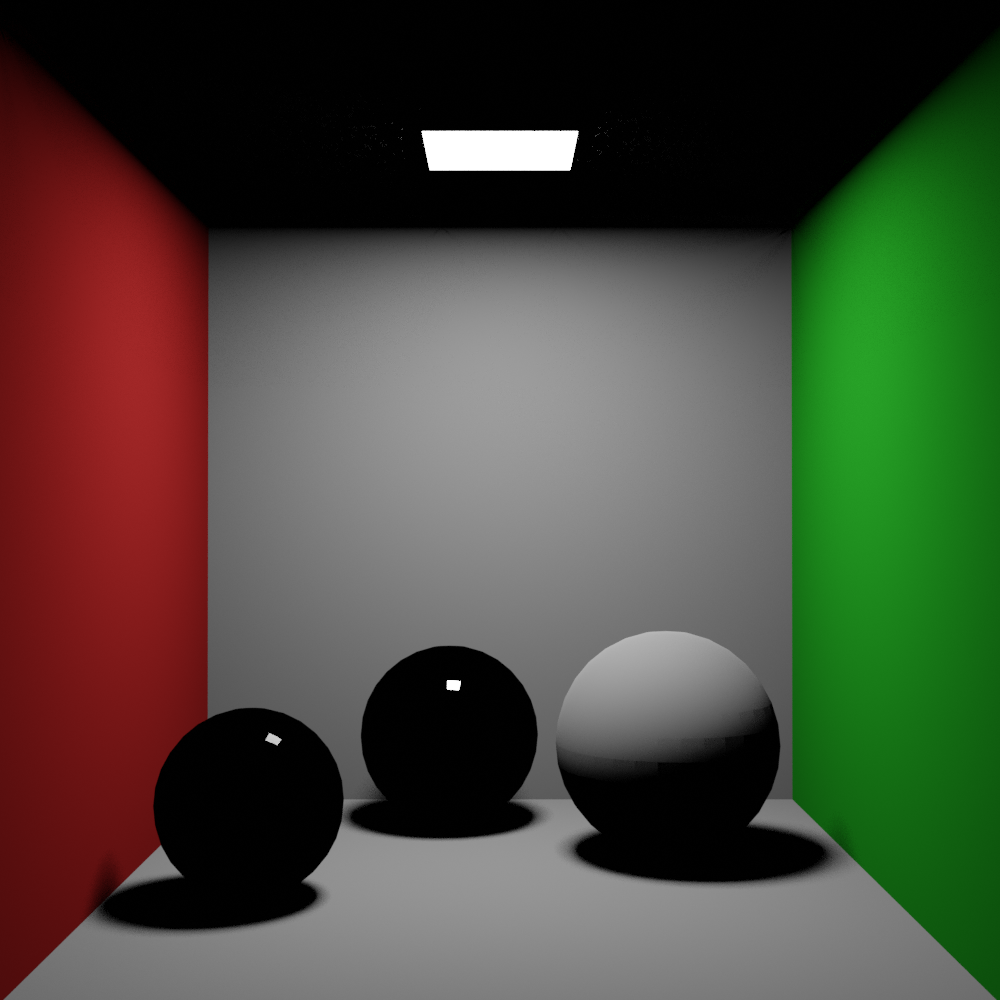
\includegraphics[width=5cm]{Figures/cornelldirect.png} }}%
  \qquad
  \subfloat[Globální osvětlovací model]{{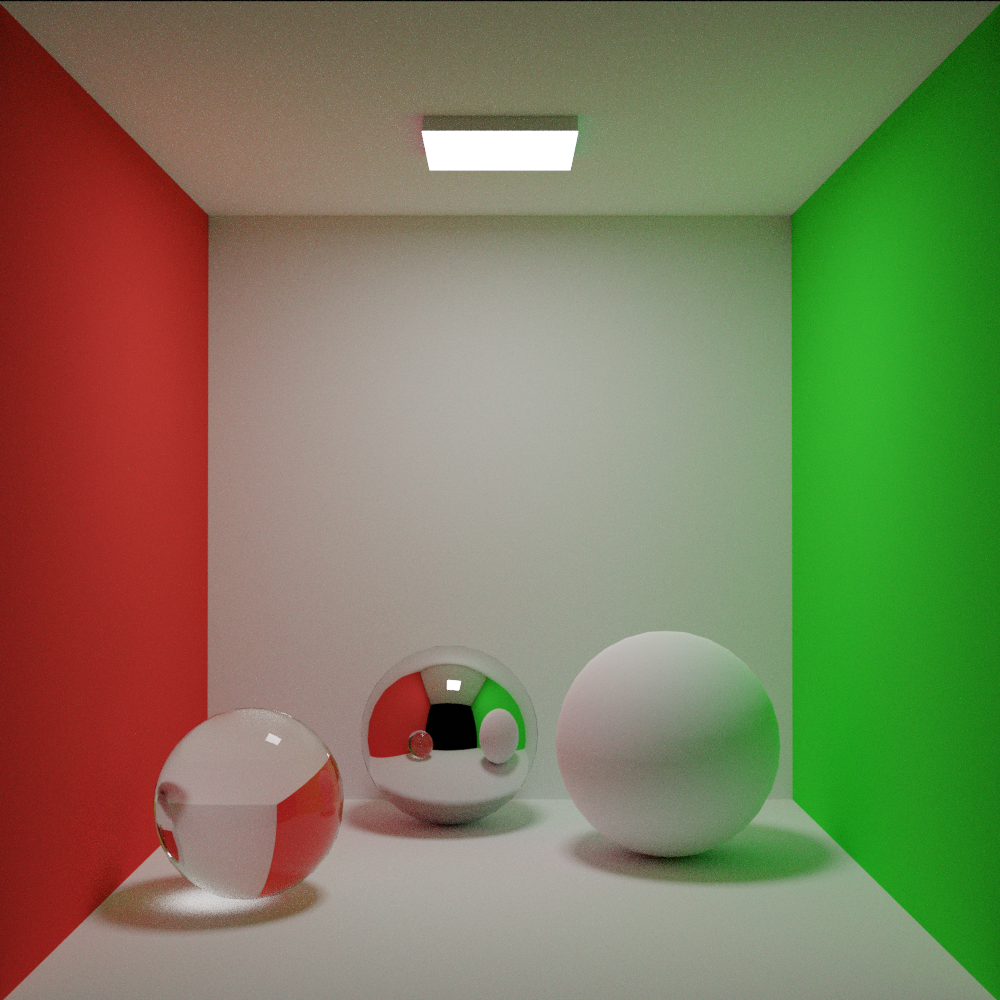
\includegraphics[width=5cm]{Figures/cornellIndirect.png} }}%
  \caption{Srovnání osvětlovacích modelů}%
  \label{fig:localVsGlobalIllum}%
\end{figure}

\subsection{Osvětlení pomocí HDR mapy}
TODO

\section{Rendering pomocí metody sledování paprsku}
Při renderingu pomocí klasických metod se postupuje pomocí standardního zobrazovacího řetězce. Postup je ve zkratce následující: Vrcholy tělesa jsou nahrány do GPU, následně se ve fragment shaderu aplikují transformačí matice a matice pro převod z lokálního do globálního prostoru. Následně je provedena rasterizace tělesa. Nakonec je ve fragment shaderu vypočítáno osvětlení tělesa. Standardní zobrazovací řetězec má tu výhodu, že je možné renderovat za běhu programu, v reálném čase. Nevýhodou ovšem je ztráta jisté reálnosti výstupu.\par
Oproti tomu při použití metody sledování paprsku je scéna protnuta s pomyslnou plochou, ze které jsou potom vysílány do scény paprsky ve formě parametrických přímek. Následně se provádí traverzace ve scéně (testování, který objekt ve scéně paprsek protnul). Při protnutí tělesa je možné následně počítat další odrazy paprsků a simulovat tak šíření světla ve scéně. Výhodou použití metody sledování paprsků je možnost velmi reálných výsledků. Nevýhodou je ale vysoká výpočetní náročnost. Výpočet komplexních scén pouze pomocí metod sledování paprsků v reálném čase je komplikovaný problém. V současné době je možná hardwarová akcelerace na grafických kartách. Pro urychlení výpočtu jsou také používány hluboké neuronové sítě (např.\ technologie Nvidia DLSS). Je možné provádět výpočet pro nižší rozlišení a následně provést upscaling (zvýšení rozlišení). Neuronová síť je schopná dopočítat chybějící data. Výsledkem je dle Nvidia obraz svou kvalitou srovnatelný s výpočtem rovnou ve vyšším rozlišení.

\section{Řešení renderovací rovnice pomocí metody Monte Carlo}
Analytické řešení renderovací rovnice je téměř nemožné kvůli obrovskému množství vlivů na výsledném integrálu. Z matematického hlediska existuje více způsobů, jak řešit integrály. Monte Carlo se opírá o tezi z teorie pravděpodobnosti, že průměr velkého počtu náhodných veličin se přiblíží střední hodnotě. Řešení renderovací rovnice pomocí metody Monte Carlo navrhuje Kajiya v~\cite{KajiyaRenderEq}. \par
Monte Carlo je stochastická metoda, v matematice často využívaná pro řešení složitějších integrálů. Metoda je založena na generování náhodných jevů, které jsou následně použity pro určení střední hodnoty výsledku. Pro řešení renderovací rovnice jsou typicky generovány náhodné směry odrazu světla. Výsledný obraz je poté tvořen průměrem určitého počtu vzorků. Typicky se u výsledných obrázků vytvořených pomocí path tracingu uvádí počet vzorků na pixel. Se zvyšujícím se počtem vzorků na pixel typicky stoupá ostrost a přesnost výsledného obrazu. S nízkým počtem vzorků je typicky obraz zatížen šumem (viz zrovnání na \hyperref[fig:samplesPpxComparison]{obrázku~\ref{fig:samplesPpxComparison}})\footnote{Výsledné renderované obrázky byly vytvořeny v programu Blender 2.92}.

\begin{figure}[ht]%
  \centering
  \subfloat[1 vzorek na pixel]{{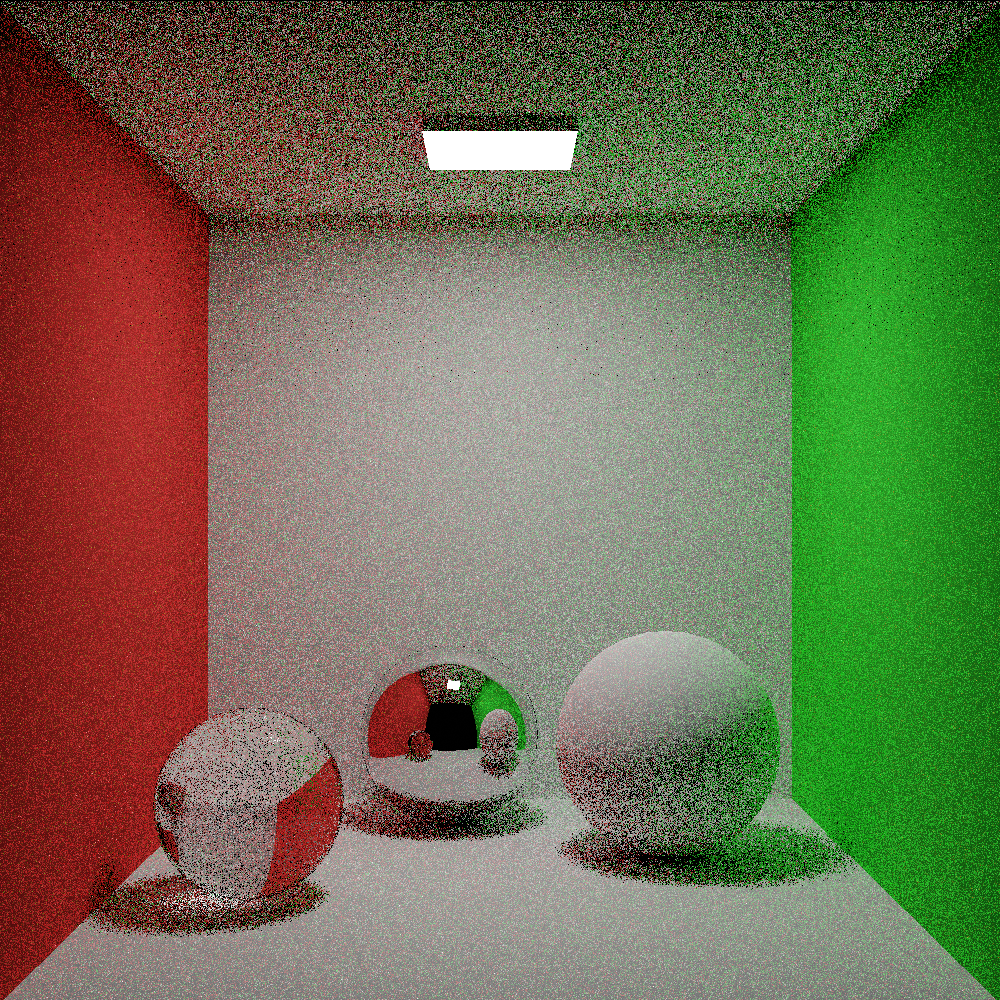
\includegraphics[width=5cm]{Figures/cornell1ppx.png} }}%
  \qquad
  \subfloat[4 vzorky na pixel]{{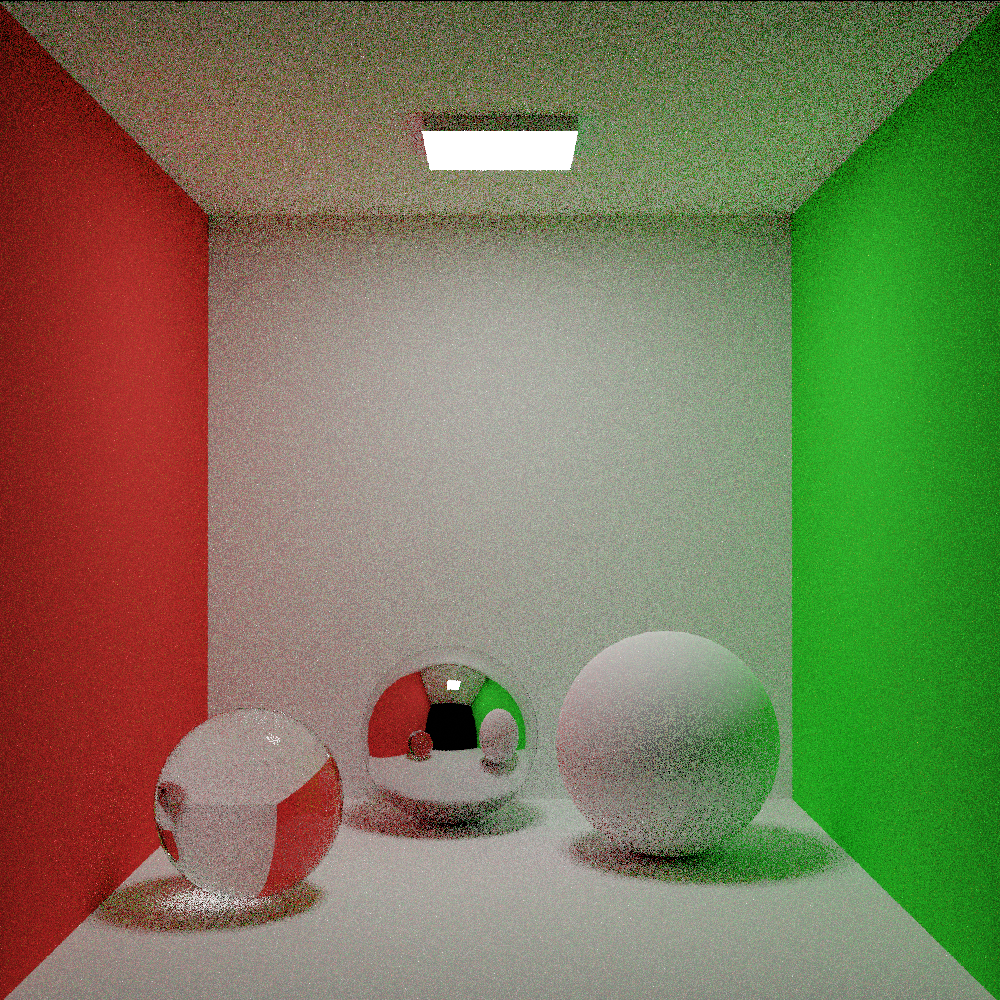
\includegraphics[width=5cm]{Figures/cornell4ppx.png} }}%
  \qquad
  \subfloat[16 vzorků na pixel]{{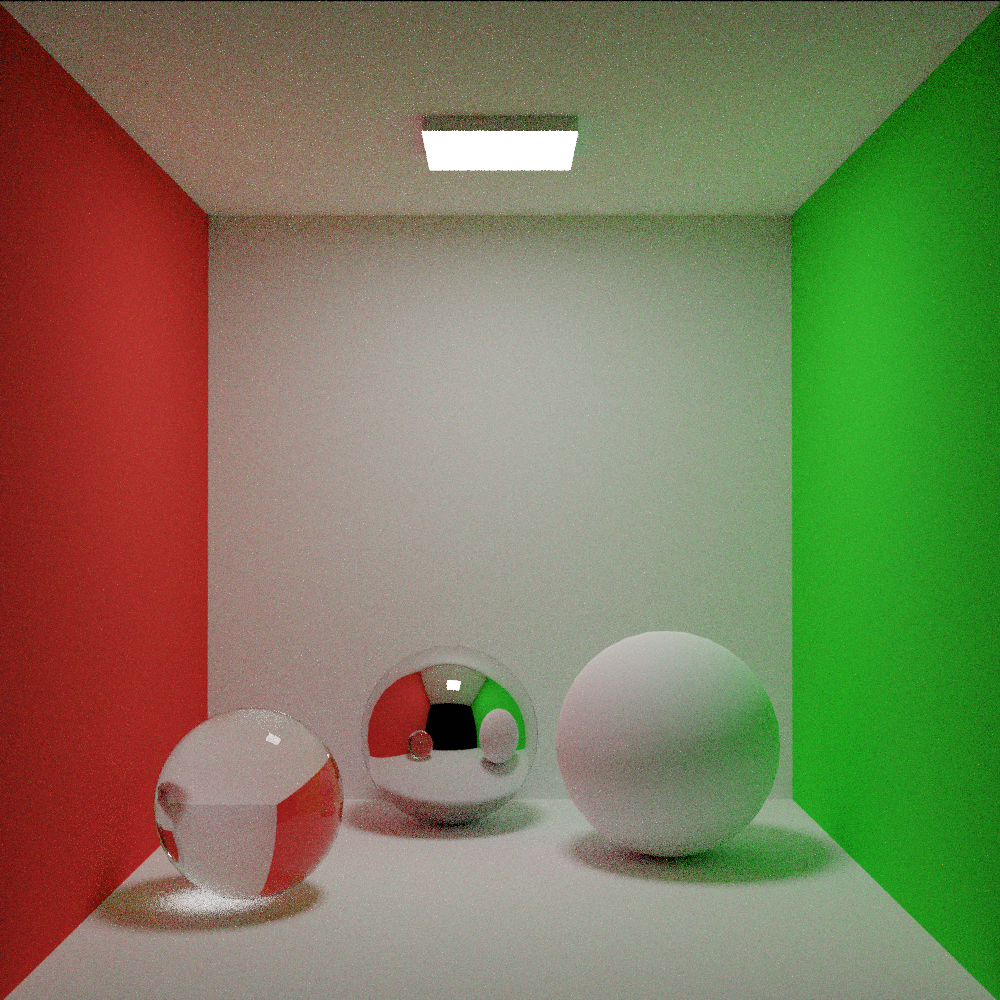
\includegraphics[width=5cm]{Figures/cornell16ppx.png} }}%
  \qquad
  \subfloat[64 vzorků na pixel]{{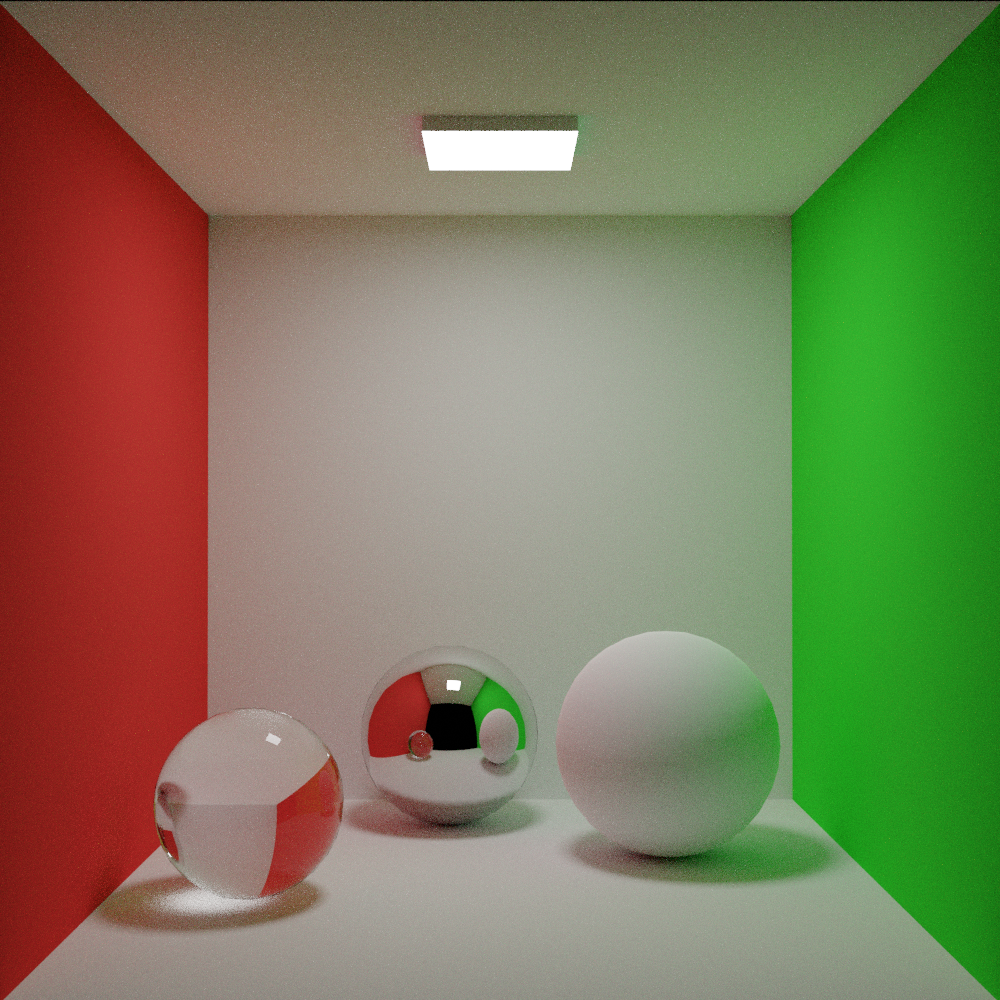
\includegraphics[width=5cm]{Figures/cornell64ppx.png} }}%
  \caption{Srovnání výsledných obrázků podle počtu vzorků na pixel}%
  \label{fig:samplesPpxComparison}%
\end{figure}

\clearpage
\chapter{BRDF}
BRDF je matematická funkce, která definuje pro daný materiál odrazivost povrchu. Určuje pro každý bod tělesa distribuci odrazu světla. Na \hyperref[fig:brdf2D]{obrázku~\ref{fig:brdf2D}} je znázorněn základní princip BRDF funkce. Vektor \(\normVec\) je normála povrchu, \(\inVec\) značí směr ke světelnému zdroji, \(\outVec\) značí směr k pozorovateli (ke kameře). BRDF je definována pro dvojici vektorů  \(\inVec\) a \(\outVec\) v daném bodě \(p\) pomocí \hyperref[eq:brdf]{vzorce~\ref{eq:brdf}}.
% Pbrt strana 350

\begin{equation} \label{eq:brdf}
  \brdf = \frac{d\outRadiance}{d\irradiance} = \frac{d\outRadiance}{\inRadiance \inDotNorm d\inVec}
\end{equation}

Je žádoucí, aby BRDF funkce splňovaly některá základní pravidla. Je důležitá  fyzikální přesnost BRDF funkce, pro kterou musí být musí být splněny následující podmínky~\cite{PHARR2017313}:
\begin{enumerate}
  % 10.3 Reciprocity 
  \item Princip vzájemnosti (Helmholtzův princip reciprocity,~\cite{hapke_2012}) --- Pro všechny dvojice \(\inVec\) a \(\outVec\) platí: \(\brdf = f_r\left(p,\inVec,\outVec\right)\)
  \item Princip zachování energie --- Celková energie odraženého světla nemůže být vyšší, než energie vstupního světla
  \item BRDF musí mít vždy nezáporný výsledek
\end{enumerate}
\begin{figure}[ht!]
  \centering
  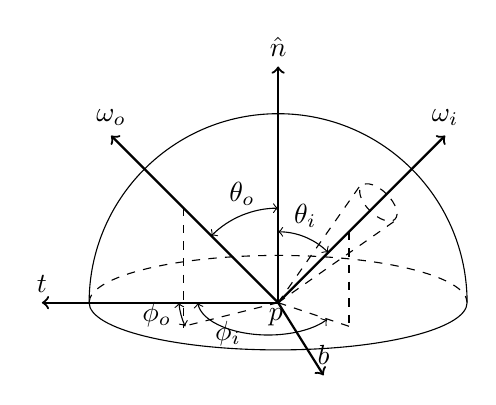
\begin{tikzpicture}[scale=0.6]
    % base circle
    \draw (-4,0) arc (180:360:4 and 1);
    \draw [dashed] (-4,0) arc (180:0:4 and 1);
    % hemisphere
    \draw (-4,0) arc (180:0:4 and 4);

    \draw [thick, ->] (0,0) -- ++(-5,0) node [at end, above] () {\(\vv{t}\)};
    \draw [thick, ->] (0,0) -- ++(135:5cm) node [at end, above] () {\(\outVec\)};
    % y
    \draw [thick, thick, ->] (0,0) -- ++(0,5) node [at end, above] () {\(\normVec\)};
    % z
    \draw [thick, ->] (0,0,0) -- ++(0,-2.5,-2.5) node [at end, above] () {\(\vv{b}\)};
    % lines spanning angle alpha
    \draw [thick, ->] (0,0) -- ++(45:5cm) node [at end, above] () {\(\inVec\)};

    \draw [thin, dashed] (0,0) -- ++(55:3cm);
    \draw [thin, dashed] (0,0) -- ++(35:3cm);

    \draw[thin, dashed, rotate=45] (3,0) ellipse (0.25cm and 0.5cm);

    \draw [thin, <->] (0,0) ++(90:1.5cm) arc (90:45:1.5cm) node [midway, above] () {\(\theta_i \)};

    \draw [thin, dashed] (1.5,1.5) -- ++(0,-2);
    \draw [thin, dashed] (0,0) -- ++(1.5,-0.5);

    \draw [thin, dashed] (-2,2) -- ++(0,-2.53);
    \draw [thin, dashed] (0,0) -- ++(-2,-0.5);

    \draw [thin, <->] (0,0) ++(180:2.1cm) arc (185:205:1.5cm) node [midway, left] () {\(\phi_o\)};

    \draw [thin, <->] (0,0) ++(180:1.7cm) arc (185:326:1.5cm and 0.75cm) node [midway, left] () {\(\phi_i \)};

    \draw [thin, <->] (0,0) ++(90:2cm) arc (90:135:2cm) node [midway, above] () {\(\theta_o\)};


    \draw (-0.05,-0.3) node () {\(p\)};
  \end{tikzpicture}
  \caption{Základní vizualizace BRDF funkce}
  \label{fig:brdf2D}
\end{figure}

\section{Přehled BRDF funkcí}\label{sec:brdffunctions}
Následující odstavce se zabývají detailním popisem a vlastnostmi jednotlivých BRDF funkcí. Budou zde vyjmenovány pouze ty BRDF funkce, které byly implementovány v praktické části této diplomové práce. \\
Pro rychlý přehled vlastností jednotlivých BRDF funkcí je možné využít \hyperref[tab:brdfProperties]{tabulku~\ref{tab:brdfProperties}} (převzato z~\cite{BRDFOverview}, zkráceno, doplněno).

\begin{table}[ht]
  \centering
  \begin{tabular}{r|lllllll}
    \hline
    BRDF model           & \rotatebox{90}{Physical} & \rotatebox{90}{Plausible} & \rotatebox{90}{Fresnel Eq}. & \rotatebox{90}{Anisotropic} & \rotatebox{90}{Sampling} & \rotatebox{90}{Rel.\ cost (cycles)} & \rotatebox{90}{Material type} \\
    \hline
    Ideal reflection     & \true                    & \true                     & \false                      & \false                      & \true                    & \(x\)                               & Mirror, perfect spec.         \\
    Lambert              & \true                    & \true                     & \false                      & \false                      & \true                    & \(x\)                               & Perfect diffuse               \\
    Phong                & \false                   & \false                    & \false                      & \false                      & \true                    & \undecided                          & Rough surf.                   \\
    Blinn-Phong          & \false                   & \false                    & \false                      & \false                      & \true                    & \(9.18x\)                           & Rough surf.                   \\
    Phys.\ correct Phong & \false                   & \true                     & \false                      & \false                      & \true                    & \undecided                          & Rough surf.                   \\
    Torrance-Sparrow     & \true                    & \false                    & \true                       & \true                       & \false                   & \undecided                          & Rough surf.                   \\
    Cook-Torrance        & \true                    & \true                     & \true                       & \false                      & \false                   & \(16.9x\)                           & Metal, plastic                \\
    Oren-Nayar           & \true                    & \true                     & \false                      & \false                      & \true                    & \(10.98x\)                          & Matte, dirty                  \\
    \hline
  \end{tabular}
  \caption{Stručný přehled implementovaných BRDF funkcí}
  \label{tab:brdfProperties}
\end{table}

\subsection{Lambert} \label{sec:Lambert}
Lambertovo BRDF (Lambertovský povrch) se řadí mezi analytické modely BRDF\@. Popisuje ideálně matné povrchy, které odráží příchozí světlo do všech směrů rovnoměrně se stejnou pravděpodobností, nehledě na příchozí směr paprsku. Jedná se o nejjednodušší BRDF funkci, je definována \hyperref[eq:lambertBRDF]{vztahem~\ref{eq:lambertBRDF}}~\cite{Koppal2014}.
%COmputer vision reference guide katushi, page 675 - Lambertian Reflectance
\begin{equation} \label{eq:lambertBRDF}
  \brdf = \frac{\alb}{\pi} = konst.
\end{equation}
\(\alb\) ve \hyperref[eq:lambertBRDF]{vztahu~\ref{eq:lambertBRDF}} vyjadřuje poměr mezi pohlceným a odraženým světlem. Tato veličina je také odborně nazývána pojmem albedo. Dělení konstantou \(\pi\) zajišťuje platnost zákona zachování energie. Díky nezávislosti na směru vstupního paprsku je také splněna reciprocita.

\begin{figure}[ht]%
  \centering\includegraphics[width=5cm]{example-image-a}%
  \caption{Vizualizace Lambertova BRDF}%
  \label{fig:lambertBRDFRender}%
\end{figure}

\subsection{Phong} \label{sec:Phong}
Phongovo BRDF vychází z Phongova osvětlovacího modelu, řadí se mezi analytické modely BRDF a používá se pro lesklé povrchy. Původní model je definován \hyperref[eq:phongBRDF]{vzorcem~\ref{eq:phongBRDF}}~\cite{Phong1975}
\begin{equation} \label{eq:phongBRDF}
  \brdf = k_s{(\refl\cdot\outVec)}^{n}
\end{equation}

Upravený, také často využívaný Blinn-Phong model je definován \hyperref[eq:blinnBRDF]{vzorcem~\ref{eq:blinnBRDF}}~\cite{BlinnPhong1977}. Výhodou upraveného Blinn-Phongova modelu oproti klasickému Phongovu modelu je hladší přechod odlesku světla.

\begin{equation} \label{eq:blinnBRDF}
  \brdf = k_s{(\normVec\cdot\halfVec)}^{n}
\end{equation}

Jak Phong, tak Blinn-Phong modely nejsou fyzikálně přesné --- nesplňují zákon zachování energie, ani zákon reciprocity~\cite{BRDFOverview}. Phongovo BRDF je možné dále upravit, aby byly splněny pravidla pro fyzikální korektnost. Fyzikálně korektní Phongovo BRDF je definováno \hyperref[eq:phongPhysicalBRDF]{vzorcem~\ref{eq:phongPhysicalBRDF}}. Pro fyzikální korektnost této varianty Phongova BRDF je potřeba dodržet \(k_d + k_s \leq 1\)~\cite{LaFortunePhongBRDF}.

\begin{equation} \label{eq:phongPhysicalBRDF}
  \brdf = \frac{k_d}{\pi} +
  \frac{k_s\left(n+2\right)}{2\pi}{\left(\cos\theta_r\right)}^{n}
\end{equation}

\begin{figure}[ht]%
  \centering
  \subfloat[Vizualizace Phongova BRDF \label{fig:phongBRDFRender}]{{\includegraphics[width=5cm]{example-image-a} }}%
  \qquad
  \subfloat[Vizualizace Blinn-Phongova BRDF \label{fig:blinnPhongBRDFRender}]{{\includegraphics[width=5cm]{example-image-b} }}%
  \qquad
  \subfloat[Vizualizace fyzikálně korektní verze Phongova BRDF \label{fig:physCorrectPhongBRDFRender}]{{\includegraphics[width=5cm]{example-image-c} }}%
  \caption{Vizualizace jednotlivých verzí Phongova BRDF}%
  \label{fig:finalrender}%
\end{figure}

\subsection{Torrance-Sparrow} \label{sec:torrancesparrow}
Torrance-Sparrow BRDF patří mezi fyzikální modely a je považován za jeden s nejúplnějších modelů~\cite{BRDFOverview}. Mimo jiné je např.\ schopen simulovat odlesk polarizovaného světla. Tento model simuluje mikroploškové materiály a pomocí parametru roughness (drsnost) simuluje mikroskopické nerovnosti materiálu. Orientace mikroskopických nerovností je v materiálu náhodná. Vyšší hodnota drsnosti materiálu snižuje lesklost materiálu. Torrance-Sparrow brdf funkce je definována \hyperref[eq:TorranceSparrow]{vzorcem~\ref{eq:TorranceSparrow}}. \par
Pro výpočet se používá distribuční funkce \(D\), která generuje rozložení normál mikroplošek. V této konkrétní implementaci je použita Beckmannova distribuční funkce (viz \hyperref[eq:beckDistr]{vzorec~\ref{eq:beckDistr}}). Beckmannova distribuční funkce pracuje s normálou mikroplošky (kolem které se generuje rozložení) a hodnotou drsnosti materiálu. Jako normála mikroplošky je použit poloviční vektor mezi pohledovým a světelným vektorem (viz \hyperref[sec:Phong]{\ref{sec:Phong} Phong}) z důvodu, že mikroploška perfektně odráží světlo právě v případě, kdy je orientovaná podél polovičního vektoru~\cite{PHARR2017507}. \par
Dále se počítá poměr odraženého světla a lomeného světla \(F\) pomocí Fresnelových vzorců. Pro výpočet je použita Schlickova aproximace (viz \hyperref[eq:schlickFresnel]{vzorec~\ref{eq:schlickFresnel}})~\cite{SchlickFresnel}. \par
Poslední část pro výpočet je koeficient geometrického útlumu \(G\), která vyjadřuje zakrytí mikroplošek při odrazu světla (viz \hyperref[eq:geomAtatenuation]{vzorec~\ref{eq:geomAtatenuation}})~\cite{BRDFOverview}.


\begin{eqnarray}
  \brdf & = & \frac{k_d}{\pi} + \frac{k_s D(\halfVec,\rough) F(\outVec) G(\outVec,\inVec)}{4\pi (\normVec \cdot \inVec)}\label{eq:TorranceSparrow}\\
  D(\halfVec,\rough) & = & \frac{e^{\left(\frac{(\normVec\cdot \halfVec)^{2}-1}{\rough^{2}(\normVec \cdot \halfVec)^{2}}\right)}}{\rough^2(\normVec\cdot \halfVec)^{2}}\label{eq:beckDistr}\\
  F(\outVec) & \approx & R(\theta) = \ior + {(1-\ior)}{(1-\cos\theta)}^{5}\label{eq:schlickFresnel}\\
  G(\outVec,\inVec) & = & \min \left( 1, \frac{2 ( \normVec \cdot \halfVec ) ( \normVec \cdot \outVec )
    }{ ( \outVec \cdot \halfVec ) },\frac{ 2 ( \normVec \cdot \halfVec ) ( \normVec \cdot \inVec ) }{ ( \outVec \cdot \halfVec ) } \right) \label{eq:geomAtatenuation}
\end{eqnarray}

\begin{figure}[ht]%
  \centering\includegraphics[width=5cm]{example-image-a}%
  \caption{Vizualizace Torrance-Sparrow BRDF}%
  \label{fig:torranceSparrowBRDFRender}%
\end{figure}

\subsection{Cook-Torrance}
Cook-Torrance BRDF rozšiřuje mikroploškové BRDF s myšlenkou, že pouze mikroplošky orientované podél vektoru \(\halfVec\) mají vliv na výsledném odrazu světla. Odrazová složka výsledného obrazu využívá pro výpočet opět funkce \(F, D, G\) (viz \hyperref[sec:torrancesparrow]{\ref{sec:torrancesparrow} Torrance-Sparrow}). Cook-Torrance BRDF se vypočítá podle \hyperref[eq:CookTorrance]{vzorce~\ref{eq:CookTorrance}}~\cite{CookTorranceBRDF}. Nevýhodou této BRDF funkce je nesplnění fyzikální přesnosti z důvodu nesplnění zákona zachování energie pro některé \(\left(\outVec,\inVec\right)\)~\cite{BRDFOverview}.

\begin{equation} \label{eq:CookTorrance}
  \brdf  = \frac{F(\outVec)}{\pi} \frac{D(\halfVec,\rough)}{(\normVec\cdot\inVec)} \frac{G(\outVec,\inVec)}{(\normVec\cdot\outVec)}
\end{equation}


\begin{figure}[ht]%
  \centering\includegraphics[width=5cm]{example-image-a}%
  \caption{Vizualizace Cook-Torrance BRDF}%
  \label{fig:cookTorranceBRDFRender}%
\end{figure}

\subsection{Oren-Nayar}
Oren-Nayar BRDF popisuje Lambertovské difusivní materiály. Oproti Lambertovu BRDF (\hyperref[sec:Lambert]{viz~\ref{sec:Lambert} Lambert}) pracuje s mikroploškami, které ale na rozdíl od mikroplošek popisovaných např.\ \hyperref[sec:torrancesparrow]{Torrance-Sparrow} modelem nejsou odrazivé, ale difuzivní. Oren-Nayar bere v úvahu odrazy světla mezi jednotlivými mikroploškami s limitovaným maximálním počtem odrazů mezi dvojicí mikroplošek. Pro generování distribuce orientace mikroplošek je použito Gaussovo rozdělení~\cite{OrenNayar}~\cite{BRDFOverview}. Oren-Nayar BRDF je definováno \hyperref[eq:OrenNayar]{vzorcem~\ref{eq:OrenNayar}}

\newcommand{\cosphiri}{\cos\left(\phi_r-\phi_i\right)}

\begin{eqnarray}
  \alpha & = & \max(\theta_i , \theta_o) = \max(\arccos(\normVec\cdot\inVec), \arccos(\normVec\cdot\outVec)) \nonumber \\
  \beta & = & \min(\theta_i , \theta_o) = \min(\arccos(\normVec\cdot\inVec), \arccos(\normVec\cdot\outVec)) \nonumber \\
  \cosphiri & = & \widehat{\left( \inVec - \normVec(\normVec\cdot\inVec) \right)} \cdot \widehat{\left( \outVec - \normVec(\normVec\cdot\outVec)  \right)} \nonumber \\
  C_1 & = & 1-0.5\frac{\rough^{2}}{\rough^{2} + 0.33} \nonumber \\
  C_2 & = & \left\{\begin{matrix*}[l] 0.45\frac{\rough^{2}}{\rough^{2}+0.09}\sin\alpha & \cosphiri \geq 0\\ 0.45\frac{\rough^{2}}{\rough^2+0.09}\left(\sin\alpha-\left(\frac{2\beta}{\pi}\right)^{3}\right) & jinak \end{matrix*}\right. \nonumber \\
  C_3 & = & 0.125\left(\frac{\rough^2}{\rough^2 + 0.009}\right)\left(\frac{4\alpha\beta}{\pi^2}\right)^{2} \nonumber \\
  L^{1}_{r} & = & \frac{\alb}{\pi}\left[C_1 + \cosphiri C_2\tan\beta + \left( 1-\left | \cosphiri  \right | \right)C_3\tan \left(\frac{\alpha+\beta}{2}\right)\right] \nonumber \\
  L^{2}_{r} & = & 0.17\frac{\alb^{2}}{\pi}\frac{\rough^{2}}{\rough^2+0.13}\left[1 - \cosphiri  \left(\frac{2\beta}{\pi}\right)^{2} \right] \nonumber \\
  \brdf & = & L^{1}_{r} + L^{2}_{r} \label{eq:OrenNayar}
\end{eqnarray}

\begin{figure}[ht]%
  \centering\includegraphics[width=5cm]{example-image-a}%
  \caption{Vizualizace Oren-Nayar BRDF}%
  \label{fig:orenNayarBRDFRender}%
\end{figure}

\subsection{Srovnání náročnosti výpočtu BRDF funkcí}
Následující kapitoly se se zabývají srovnáním jednotlivých BRDF funkcí dle jejich výpočetní složitosti.
\subsubsection{Metodika výpočtu výpočetní složitosti}
Při výpočtu složitosti jsem se rozhodl pro praktické měření výkonu jednotlivých algoritmů, protože výsledná hodnota má pro praktickou implementaci vyšší informační hodnotu, než teoretická analýza. Jako metriku jsem zvolil absolutní a relativní čas výpočtu řádově \(10^7\) iterací výpočtu. Výsledky měření jsem pak rozdělil do tří kategorií - celkové srovnání, srovnání BRDF funkcí pro difuzní povrchy a srovnání BRDF funkcí pro lesklé povrchy.

\subsubsection{Výsledky měření, zhodnocení}
Konkrétní výsledky měření jsou uvedeny v tabulkách \hyperref[tab:DiffuseBRDFsComparison]{\ref{tab:DiffuseBRDFsComparison}}, \hyperref[tab:GlossyBRDFsComparison]{\ref{tab:GlossyBRDFsComparison}} a \hyperref[tab:AllBRDFsComparison]{\ref{tab:AllBRDFsComparison}}.  Z výsledků z \hyperref[tab:DiffuseBRDFsComparison]{tabulky \ref{tab:DiffuseBRDFsComparison}} vyplývá, že Lambertovo BRDF je z hlediska výpočetního výkonu nejefektivnější BRDF funkce. Tento výsledek je očekávatelný, už z důvodu velmi jednoduchého vzorce. Oproti Lambertovu BRDF ale Oren-Nayar poskytuje širší možnosti nastavení díky parametru drsnosti. Oren-Nayar tak může věrněji reprezentovat drsnější difuzivní materiály.\par
Ze srovnání BRDF funkcí pro lesklé povrchy v \hyperref[tab:GlossyBRDFsComparison]{tabulce \ref{tab:GlossyBRDFsComparison}} vyplývá, že mezi jednotlivými funkcemi není rozdíl příliš markantní. Pozornost si zaslouží rozdíl mezi tradičním Phongovým BRDF a jeho fyzikálně přesnou variantou. Je vidět, že přidáním fyzikální korektnosti se výkon zhoršil pouze o cca \(16\%\).


\begin{table}[ht]
  \centering
  \begin{tabular}{r|ll}
    BRDF funkce & Absolutní čas & Relativní čas \\
    \hline
    Lambert     & 0.0470865s    & 1             \\
    Oren Nayar  & 1.75046s      & 37.1755
  \end{tabular}
  \caption{Srovnání BRDF funkcí pro difuzní povrchy}
  \label{tab:DiffuseBRDFsComparison}
\end{table}

\begin{table}[ht]
  \centering
  \begin{tabular}{r|ll}
    BRDF funkce              & Absolutní čas & Relativní čas \\
    \hline
    Phong                    & 0.402189s     & 1             \\
    Blinn Phong              & 0.445108s     & 1.10671       \\
    Physically correct Phong & 0.46521s      & 1.15669       \\
    Torrance sparrow         & 0.520102s     & 1.29318
  \end{tabular}
  \caption{Srovnání BRDF funkcí pro lesklé povrchy}
  \label{tab:GlossyBRDFsComparison}
\end{table}

\begin{table}[ht]
  \centering
  \begin{tabular}{r|ll}
    BRDF funkce              & Absolutní čas & Relativní čas \\
    \hline
    Lambert                  & 0.0470865s    & 1             \\
    Phong                    & 0.402189s     & 8.54149       \\
    Blinn Phong              & 0.445108s     & 9.45298       \\
    Physically correct Phong & 0.46521s      & 9.87989       \\
    Torrance sparrow         & 0.520102s     & 11.0457       \\
    Oren Nayar               & 1.75046s      & 37.1755
  \end{tabular}
  \caption{Celkové srovnání všech BRDF funkcí}
  \label{tab:AllBRDFsComparison}
\end{table}




\clearpage
\chapter{Vizualizační aplikace}
Aplikace jako taková umožňuje zobrazit BRDF funkce popsané v kapitole \hyperref[sec:brdffunctions]{\ref{sec:brdffunctions} Přehled BRDF funkcí}. Důležitým prvkem je také interaktivita, kdy je možné měnit jednotlivé parametry BRDF funkcí. Kromě samotných BRDF funkcí aplikace umožňuje zobrazit i metody pro vzorkování funkcí (toto téma je dále rozebráno v kapitole \hyperref[sec:reduction]{\ref{sec:reduction} Redukce variance Monte Carlo}), kdy je možné přepínat mezi jednotlivými BRDF funkcemi a vzorkovacími funkcemi. Je tedy možné demonstrovat důležitost správného výběru vzorkovací funkce k vybrané BRDF funkci. Pro doplnění funkcionality obsahuje aplikace také možnost pro uložení snímku aktuální vizualizace BRDF ve vysokém rozlišení. \par
Poslední funkcionalitou je interaktivní okno s jednoduchou scénou, která je renderována s použitím aktuálně vybrané BRDF funkce. Pro jednoduchost je renderován model koule, která je popsána analyticky. Tato testovací scéna je primárně osvětlena HDR obrazem, ale aplikace také umožňuje osvětlit scénu konstantním jasem. Tímto nastavením je simulována situace, kdy na objekt dopadá ze všech směrů stejné množství světla. Takto osvětlená scéna je známa jako tzv. Furnace test a slouží pro kontrolu fyzikální korektnosti BRDF funkce.\par
Následující odstavce se zabývají konkrétními detaily implementace a popisem technických řešení použitých pro jednotlivé funkce implementované vizualizační aplikace.

\section{Existující řešení}
Existuje množství aplikací řešících podobnou tematiku. V zásadě lze tyto aplikace rozdělit do dvou kategorií:
\begin{enumerate}
  \item Aplikace pro zobrazení BRDF funkcí
  \item Aplikace pro návrh BRDF funkcí
\end{enumerate}
Aplikace vytvořená v této práci spadá do první kategorie, primárně se zabývá pouze zobrazováním. V následujících odstavcích jsou popsány vybrané aplikace z obou kategorií.

\subsection{Aplikace pro zobrazení BRDF funkcí}
Ve článku~\cite{DisneyBRDF} byla představena aplikace Disney BRDF Explorer\footnote{\url{https://github.com/wdas/brdf}}. Aplikace umí načítat a srovnávat analyticky zadané BRDF modely. Aplikace také umí načítat a zobrazovat BRDF modely popsané pomocí měření (např.\ z MERL\footnote{\url{https://www.merl.com/brdf/}} databáze), umí také zobrazit finální render s použitím zvolené BRDF funkce. Aplikace je licencována jako open-source, je multiplatformní a používá pro svou funkcionalitu knihovnu QT\@. Pro rendering je použita technologie OpenGL\@.\par
Článek~\cite{brdfviz} se zabývá implementací systému pro vizualizaci BRDF funkcí dostupných v databázi \textquote{Oregon BRDF Library}\footnote{\url{https://math.nist.gov/~FHunt/appearance/obl.html}}. Aplikace je implementována za pomocí knihovny AVS Express. Výsledná aplikace není veřejně dostupná.

\subsection{Aplikace pro návrh BRDF funkcí}
Ve článku~\cite{Fors2009BRDFLabAG} je popsána aplikace BRDFLab\footnote{\url{http://brdflab.sourceforge.net/}} pro vizualizaci BRDF funkcí zadaných analyticky, pomocí nameřených dat, nebo pomocí dat získaných simulací. Také je možné vytvořit BRDF funkce kombinací analyticky zadaných, předpřipravených laloků. Aplikace také umožňuje vizualizaci finálního renderu s použitím BRDF funkce. Aplikace je distribuována jako open-source, pro GUI je použita knihovna QT, pro rendering je použita knihovna Ogre3D.
\par
Článek~\cite{brdfshop} se zabývá popisem aplikace BRDF-Shop, která je primárně určena pro návrh BRDF funkcí založených na Wardově BRDF\@. Aplikace jako taková je implementována jako plugin do 3D editoru Autodesk Maya. APlikace nemá možnost zadání BRDF funkce analyticky.

\section{Vizualizace BRDF}
Při implementaci jsem se chtěl co nejvíce přiblížit standardním referenčním obrázkům popisujícím princip BRDF funkcí (viz \hyperref[fig:brdf2D]{obrázek~\ref{fig:brdf2D}}). Výsledná vizualizace znázorňuje  pro daný vstupní směr všechny možné výstupní směry, do kterých se světlo odráží. Této vizualizace se dá jednoduše dosáhnout tak, že se vygeneruje jednotková hemisféra a jednotlivé body na hemisféře jsou posunuty o hodnotu BRDF funkce pro daný vstupní a výstupní směr. Každý bod na hemisféře zvýrazňuje výstupní směr, vzdálenost bodu od středu (délka vektoru) zvýrazňuje hodnotu BRDF funkce. \par
Pro vizualizaci jsem se rozhodl vygenerovat jednotkovou polokouli a jednotlivé body polokoule upravit v OpenGL Vertex shaderu. Při generování polokoule jsem narazil na problém, kdy pro vizualizaci bylo potřeba mít co nejrovnoměrněji rozložené polygony, ideálně všechny s podobnou velikostí. Rozhodl jsem se tedy negenerovat UV kouli, ale geodetický mnohostěn (srovnání na \hyperref[fig:spheresComparison]{obrázku~\ref{fig:spheresComparison}}), který je tvořen rovnostrannými trojúhelníky.  \par

\begin{figure}[ht]
  \centering
  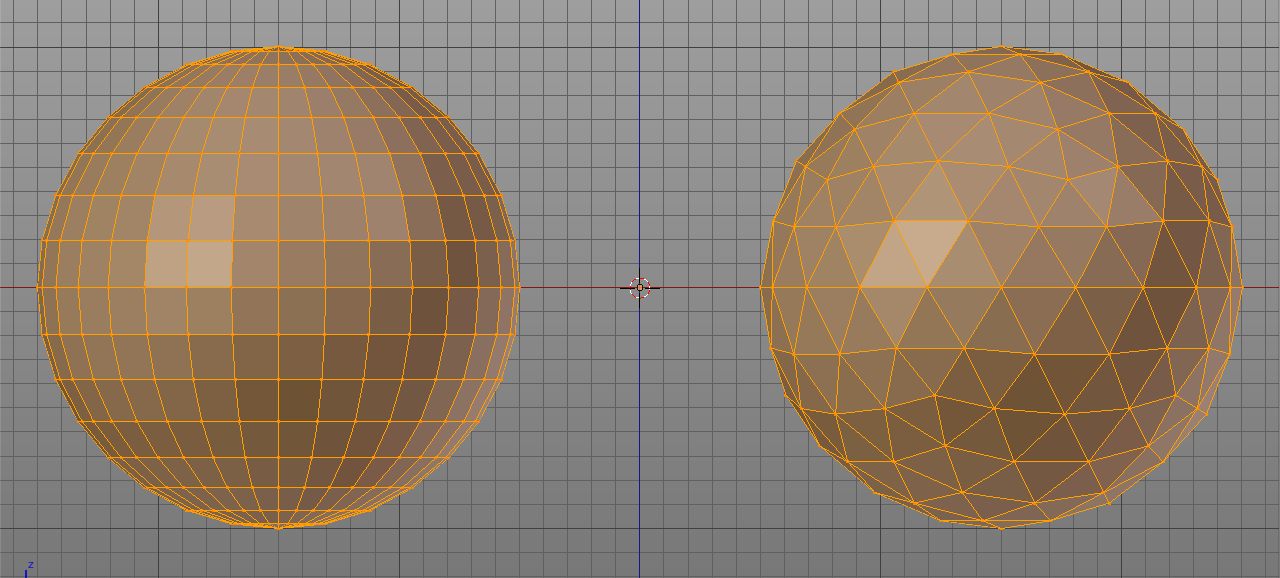
\includegraphics[width=10cm]{Figures/IcosphereUVSphereComparison.png}
  \caption{Srovnání UV koule a geodetického mnohostěnu, z~\cite{tan_2019}}
  \label{fig:spheresComparison}
\end{figure}
Pro zjednodušení implementace jsem vycházel z kódu pro dvacetistěn~\cite{OpenGLSphere}, jehož trojúhelníkové stěny jsem dále rekurzivně dělil. Počet rekurzivních dělení určuje rozlišení výsledné vizualizace, s vyšším počtem dělení se zvyšuje rozlišení. Postup generování hemisféry použité pro vykreslení BRDF funkcí je zobrazen na \hyperref[fig:hemisfera]{obrázku~\ref{fig:hemisfera}}.\par

\begin{figure}[ht]%
  \centering
  \subfloat[Dvacetistěn \label{fig:icasehedron}]{{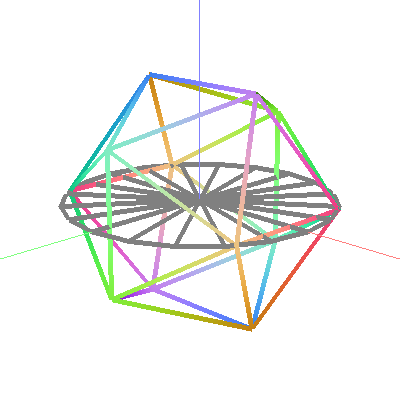
\includegraphics[width=5cm]{Figures/icosphere.png} }}%
  \qquad
  \subfloat[Poloviční dvacetistěn \label{fig:halficasehedron}]{{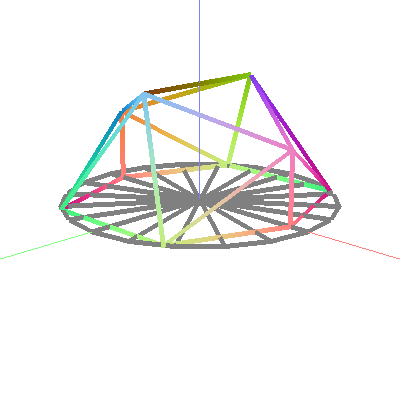
\includegraphics[width=5cm]{Figures/halficosphere.png} }}%
  \qquad
  \subfloat[Poloviční dvacetistěn, \(1\times\) rozdělené polygony \label{fig:halficasehedron1}]{{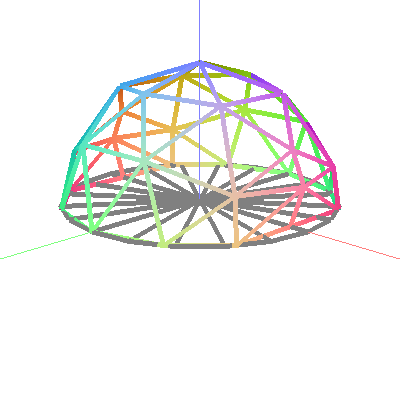
\includegraphics[width=5cm]{Figures/halficosphere1.png} }}%
  \qquad
  \subfloat[Poloviční dvacetistěn, \(3\times\) rozdělené polygony \label{fig:halficasehedron3}]{{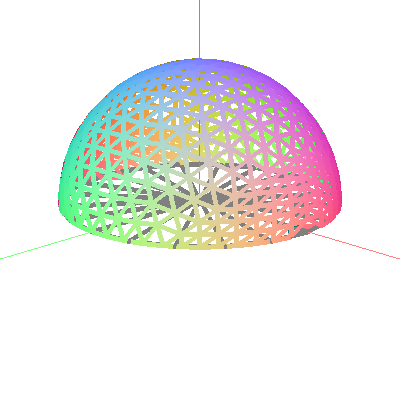
\includegraphics[width=5cm]{Figures/halficosphere3.png} }}%
  \caption{Postup generování hemisféry}%
  \label{fig:hemisfera}%
\end{figure}

Body takto generované hemisféry jsou následně upraveny ve vertex shaderu. Základní kód pro úpravu hemisféry glsl vertex shaderem je uveden ve \hyperref[src:vertexbrdf]{výpise~\ref{src:vertexbrdf}}. Vertex shader pracuje se vstupními parametry \texttt{in\_Position}, \texttt{u\_incidentVector} a parametry pro jednotlivé BRDF funkce. Pro jednoduchost je výpis zkrácen a zjednodušen. Parametr \texttt{in\_Position} určuje vstupní bod hemisféry a před vstupem do brdf funkce je normalizován (aby byla pojištěna jednotková vzdálenost od středu). Parametr \texttt{u\_incidentVector} představuje směrový vektor \(\outVec\). \par

\begin{listing}[ht]
  \inputminted{c++}{sampleshader.glsl}
  \caption{Zjednodušený vertex shader}
  \label{src:vertexbrdf}
\end{listing}

Ve vertex shaderu jsou poté ve funkci \texttt{BRDF()} implementovány jednotlivé BRDF funkce. Pro přepínání mezi aktuálně zvolenou BRDF funkcí slouží uniformní proměnná, která je do shaderu předávána z programu. Parametry jednotlivých funkcí jsou také předávány pomocí uniformních proměnných. Po zpracování ve vertex shaderu je následně vizualizace zpracována fragment shaderem, kde je každý bod vizualizace jednoduše obarven podle vzdálenosti bodu od středu (tzn.\ dle hodoty BRDF funkce daného bodu). Obarvení dané hodnoty BRDF funkce je provedeno za pomocí sekvenční barevné mapy \textit{YLGnBu}. Ukázka výsledné vizualizace je zobrazena na \hyperref[fig:brdfExample]{obrázku~\ref{fig:brdfExample}}, kde je vizualizována fyzikálně korektní Phongova BRDF funkce.

\begin{figure}
  \centering
  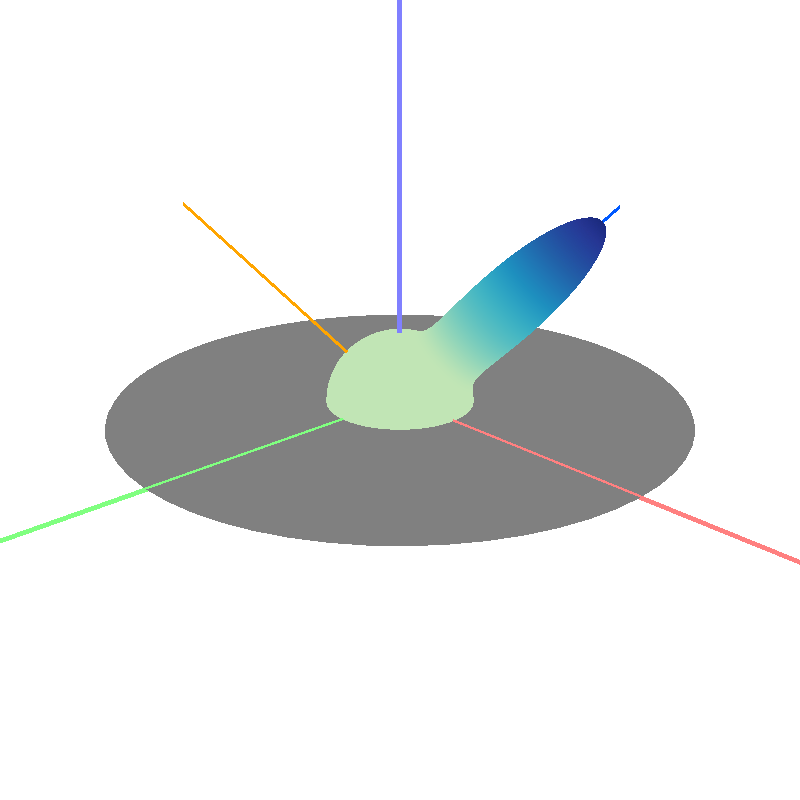
\includegraphics[width=6cm]{Figures/brdfVizExample.png}
  \caption{Ukázka vizualizace BRDF}%
  \label{fig:brdfExample}%
\end{figure}

\section{Vizualizace vzorkování}
Každou BRDF funkci je vhodné kombinovat s vhodně zvolenou vzorkovací funkci. Vzorkovací funkce jsou podrobněji popsány v kapitole \hyperref[sec:reduction]{\ref{sec:reduction} Redukce variance Monte Carlo}. K vizualizaci vzorkovacích funkcí jsem se rozhodl přistoupit pomocí vizualizace vektory. Princip je v zásadě jednoduchý. Vzorkovací funkce pracují tak, že se vygeneruje směr pro náhodně vygenerované hodnoty \(\randU\) a \(\randV\). Vizualizace potom funguje na principu vygenerování uniformně rozložených hodnot v mřížce s daným rozlišením. Takto generované hodnoty jsou poté převedeny pomocí vzorkovací funkce do vektorů. Uniformně rozložené generované vektory jsou poté přímo zobrazeny. V případě potřeby je možné interaktivně zvýšit nebo snížit počet vzorků. Ve výchozím nastavení je délka jednotlivých vizualizovaných vektorů jednotková. Je také možné nastavit násobení velikostí vektorů hodnotou pdf. Násobení velikosti vektoru hodnotou pdf demonstruje rozložení pravděpodobnosti vzorku. Čím větší je velikost vzorku, tím větší je jeho pravděpodobnost. Na \hyperref[fig:samplingExample]{obrázku~\ref{fig:samplingExample}} je zobrazena ukázka vizualizace vzorkovací funkce.

\begin{figure}
  \centering
  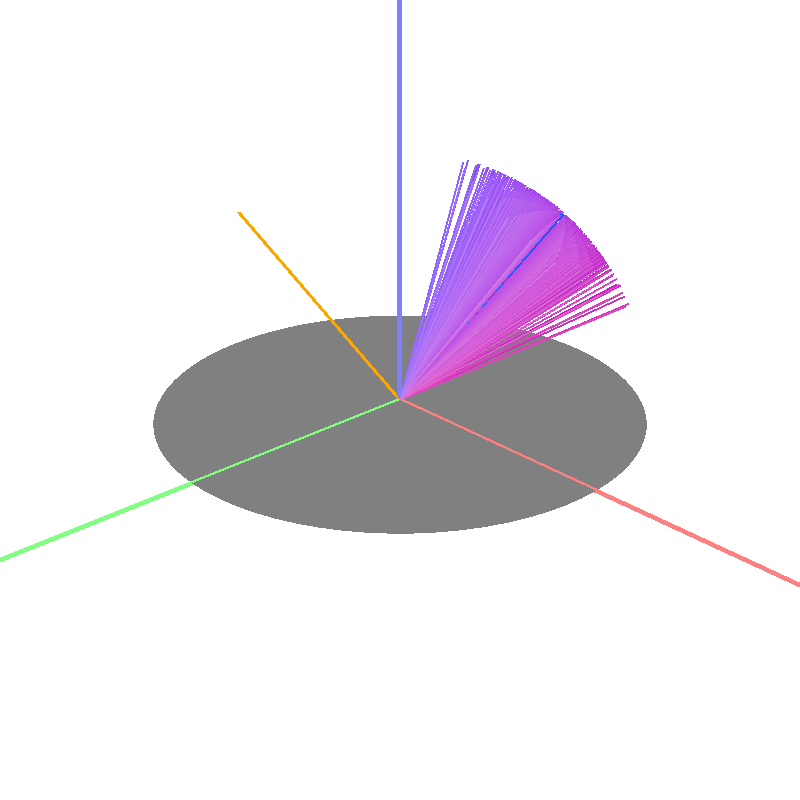
\includegraphics[width=6cm]{Figures/samplingExample.png}
  \caption{Ukázka vizualizace vzorkování}%
  \label{fig:samplingExample}%
\end{figure}


\section{Vizualizace výsledného renderu}
Pro ukázku výsledku je vizualizován také výsledný render. Jak již bylo zmíněno, vizualizována je koule, která je osvětlena HDR mapou, nebo konstantním pozadím. \par
Pro výpočet osvětlení je využita metoda Monte Carlo, v path traceru jsou také implementovány funkce pro optimalizaci výpočtu. Pro ukázku volby vzorkovací funkce využívá path tracer vzorkovací funkci zvolenou v ovládacím panelu. Jednotlivé vzorkovací funkce jsou podrobněji popsány v kapitole \hyperref[sec:reduction]{\ref{sec:reduction} Redukce variance Monte Carlo}. Implementováno je také vzorkování světelných zdrojů z HDR mapy. Vzorkování světelných zdrojů je možné v ovládacím panelu zapínat a vypínat, pro demonstraci efektů jednotlivých typů vzorkování na výsledném renderu. \par
Kromě analyticky zadané koule je také možné vizualizovat render libovolného načteného objektu. Pro urychlení výpočtu je načtený objekt uložen do BVH stromu --- akcelerační struktury, dále popsané v kapitole \hyperref[sec:reduction]{\ref{sec:reduction} Redukce variance Monte Carlo}. Výsledek renderu je zobrazen na obrázcích \hyperref[fig:loadedObjectRender]{\ref{fig:loadedObjectRender}} a \hyperref[fig:analSphereObjectRender]{\ref{fig:analSphereObjectRender}}.

\begin{listing}[ht]
  \inputminted{python}{pathTracer.py}
  \caption{Pseudokód pro path tracer}
  \label{src:pathtracer}
\end{listing}

\begin{figure}[ht]%
  \centering
  \subfloat[Render načteného objektu \label{fig:loadedObjectRender}]{{\includegraphics[width=5cm]{example-image-a} }}%
  \qquad
  \subfloat[Render analyticky zadané koule \label{fig:analSphereObjectRender}]{{\includegraphics[width=5cm]{example-image-b} }}%
  \caption{Ukázka vizualizace výsledného renderu}%
  \label{fig:finalrender}%
\end{figure}

\section{Detaily implementace aplikace, použité knihovny a technologie}
Aplikace pro vizualizaci je napsána v moderním C++, s použitím standardu C++17. Při implementaci jsem se snažil v maximální možné míře využívat novou funkcionalitu tohoto standardu. \par
Co se týče architektury mého řešení, je aplikace rozdělena do tří samostatných celků. Hlavní částí aplikace je samotné uživatelské rozhraní, ve kterém jsou všechny ovládací panely. Přímé vykreslování do panelů definovaných knohovnou ImGui není možné, vykreslování jsem tedy prováděl do frame bufferu, resp.\ do textury. Samotné textury jsem poté zobrazoval v ImGui panelech. \par
OpenGL část aplikace se zabývá samotným vykreslováním BRDF funkcí a vzorkování. \par
Embree část aplikace je zodpovědná z vykreslování objektu za pomocí zvolené BRDF funkce.
\subsection{Použité knihovny}
Následující kapitoly se věnují popisu knihoven, které jsem použil při implementaci své diplomové práce. Kromě popisu daných knihoven jsem také zdůvodnil použití těchto knihoven.
\subsubsection{OpenGL}
OpenGL je standardní rozhraní pro vykreslování počítačové grafiky. OpenGL je multiplatformní, je možné s ním pracovat pomocí množství programovacích jazyků a má velmi kvalitní dokumentaci. Jeho nevýhodou může být jeho neobjektový přístup. Práce s OpenGL je v podstatě globální. V současné době je OpenGL nahrazována novějším rozhraním Vulkan, které má oproti OpenGL blíže k samotnému hardwaru. Oproti OpenGL také např.\ podporuje paralelismus, současná verze už v základu podporuje ray tracing. Pro zpracování této práce byla zvoleno rozhraní OpenGL z důvodu, že nebyly potřeba nové funkce z Vulkanu.
\subsubsection{Glad}
Jak už bylo zmíněno v předchozím odstavci, OpenGL je v podstatě pouze rozhraní, standard. Je teda potřeba používat nějakou konkrétní implementaci tohoto rozhraní pro konkrétní hardware a konkrétní operační systém. Za tuto implementaci jsou zodpovědné přímo ovladače grafické karty. Pro Windows jsou primárně ovladače dodávány přímo výrobcem grafické karty. Na Linuxu jsou kromě proprietárních ovladačů od výrobců dostupné i komunitní, open-source ovladače. Vzhledem k velké diverzitě všech těchto možností kdy v době kompilace není známa přesná kombinace, je třeba tuto skutečnost nějakým způsobem ošetřit v kódu. \par
Pro zjednodušení práce s OpenGL existuje množství knihoven, které zjednodušují přístup k funkcím OpenGL\@. Pro svou diplomovou práci jsem zvolil knihovnu Glad\footnote{\url{https://github.com/Dav1dde/glad}}, která je multiplatformní a je distribuována s open-source licencí. Konfigurace této knihovny je poněkud nestandardní, Glad poskytuje webovou službu, kde je možné nakonfigurovat konkrétní požadovanou verzi a seznam požadovaných rozšíření OpenGL\@. Po konfiguraci je možné stáhnout generované zdrojové soubory. Kromě možnosti generování souborů pomocí webové služby je také možné používat knihovnu jako submodul pro CMake. V takovém případě jsou v konfigurační fázi automaticky staženy generované soubory podle daného nastavení.
\subsubsection{Glfw}
Kromě samotného rozhraní pro práci s OpenGL je také potřeba nějakým způsobem zobrazit výstup uživateli. K tomu je potřeba vytvořit okno. Pro práci s okny existuje množství knihoven, pro tuto diplomovou príci byla vybrána knihovna Glfw\footnote{\url{https://github.com/glfw/glfw}}. Kromě tvorby a práce s okny tato knihovna také podporuje pro práci s uživatelskými vstupy. \par
Výhodou knihovny Glfw je primárně odlehčenost celé knihovny. Glfw je také šířena s open-source licencí. Glfw je multiplatformní, s podporou pro všechny běžné operační systémy.

\subsubsection{Dear ImGui}
Jak již bylo zmíněno, knihovna Glfw poskytuje pouze rozhraní pro práci s okny. To znamená, že nepodporuje samotnou tvorbu uživatelského rozhraní. Pro tvorbu uživatelských rozhraní je teda potřeba použít jinou knihovnu. \par
Pro tvorbu uživatelských rozhraní existuje pro jazyk C++ velké množství různých knihoven. V různých linuxových distribucích jsou v podstatě standardem primárně dvě knihovny: QT a GTK\@. Obě knihovny jsou multiplatformní, ale ani jedna není úplně vhodná pro mé použití.\par Knihovna QT není příliš vhodná z důvodu velikosti této knihovny. QT v zásadě není jen knihovna specializovaná pouze na uživatelská rozhraní, ale je to velmi komplexní a obsáhlý framework. Pro velmi jednoduchou aplikaci, jako je aplikace implementovaná v této diplomové práci by byla většina funkcionality zbytečná. Knihovna QT také nepřináší žádnou výhodu oproti použitému řešení.\par
Oproti tomu knihovna GTK je knihovna, která se primárně zabývá tvorbou uživatelských rozhraní. Je však primárně vyvíjena pro použití na Linuxu a přestože je multiplatformní a je možné ji použít na Windows, použití na windows není primárně bráno v potaz. Knihovna GTK je také poněkud složitější na používání. \par
Po zhodnocení možností jsem se nakonec rozhodl použít knihovnu Dear ImGui\footnote{\url{https://github.com/ocornut/imgui}}. Výhodou použití této knihovny je primárně její jednoduchost použití. Do již existujícího kódu je velmi snadno integrovatelná. Samotná tvorba uživatelského rozhraní je intuitivní a přímočaré. Neexistuje oficiálně žádný grafický editor (přestože existují komunitní editory), ale knihovna je pro používání natolik jednoduchá, že takový editor ani není potřeba. Dear ImGui je možné používat nejen s OpenGL, ale i s jinými rozhraními pro počítačovou grafiku (mimo jiné kromě OpenGL oficiálně podporuje Vulkan, Metal, nebo DirectX). Dear ImGui také poskytuje množství ukázkových programů, které jsou vytvořeny pro různé kombinace platforem, použitých technologií a knihoven, ze kterých je možné vycházet. \par
Knihovna Dear ImGui je distribuována s open-source licencí a je multiplatformní. Kromě základní verze této knihovny existuje také separátní verze s podporou pro \textquote{docking} jednotlivých panelů do pracovní plochy aplikace. Pro svou diplomovou práci jsem zvolil právě tuto verzi knihovny.

\subsubsection{Glm}
Obecně v počítačové grafice se velmi často pracuje s vektory, maticemi a operacemi s nimi. Z hlediska výkonu je kritické, aby vektorové a maticové operace byly co nejvíce optimalizované. Z tohoto důvodu jsem se rozhodl pro práci s vektory a maticemi použít knihovnu Glm\footnote{\url{https://github.com/g-truc/glm}}. Knihovna Glm se velmi jednoduše používá, je distribuována pod open-source licencí a je multiplatformní. Knihovna Glm je implementována tak, aby splňovala standard jazyka GLSL, používaném v OpenGL shaderech. Není však na OpenGL závislá a lze tak tuto knihovnu použít i pro jiné účely, než jen pro počítačovou grafiku.

\subsubsection{Assimp}
Aplikace má možnost načítat uživatelské modely pro náhled renderu a nahradit tak výchozí analyticky zadaný model koule. Pro samotné načítání modelů jsem použil knihovnu Assimp\footnote{\url{https://github.com/assimp/assimp}}. Knihovna Assimp je distribuována s 3-bodovou BSD licencí. \par
Pro zjednodušení je ve výchozím stavu vypnuta většina funkcionality této knihovny, podporováno jsem ve výchozím stavu nechal pouze načítání modelů ve formátu Wavefront obj. Vypnutá funkcionalita lze jednoduše opět zapnout při konfiguraci CMake projektu. Kromě načtení modelu se načítají také materiály. Načtené materiály ale nejsou použity, protože aplikace pracuje s jedním globálním materiálem.

\subsubsection{FreeImage}
Aplikace umožňuje práci s obrázky -- načítání textur a ukládání snímků z vizualizace BRDF funkce i vizualizace finálního renderu. K tomuto účelu jsem použil rozhraní knihovny FreeImage\footnote{\url{https://freeimage.sourceforge.io/}}.

\subsubsection{Embree}
Jelikož součástí aplikace je i náhled na výsledný render pomocí path tracingu, použil jsem pro zjednodušení práce knihovnu Embree\footnote{\url{https://github.com/embree/embree}}, která se stará o tvorbu samotných paprsků a následnou traverzaci paprsku a scény. Jelikož primárně je renderován analyticky zadaný model koule, implementoval jsem nad knihovnou Embree i drobné rozhraní pro použití jak načtených modelů, tak analytických těles. Analyticky zadaná tělesa i načtené modely je tak možné používat v jedné scéně. \par
Knihovna Embree je spravována organizací Intel, je multiplatformní a distribuována s open-source licencí. Knihovna je optimalizována pro použití s Intel procesory. Nejlepšího výkonu je možné dosáhnout s procesory podporujícími AVX instrukce a při použití Intel kompilátoru. \par
Pro path tracing je možné využívat spoustu jiných knihoven s výpočtem jak na CPU, tak na GPU\@. Je možné používat např.\ přímo Vulkan pro použití na grafické kartě, případně Nvidia OptiX s výpočty také na grafické kartě, rozhodl jsem se pro Embree z důvodu nižších systémových požadavků. Výsledná aplikace je tedy funkční i na méně výkonných počítačích. Zároveň path tracing není primární funkcionalita mé diplomové práce a lze tak použít radši řešení s vyšší kompatibilitou, než s vyšším výkonem (za cenu nižší kompatibility).

\subsubsection{Spdlog}
Při vývoji aplikace je velmi užitečné používat různé informační výpisy. Informační výpisy mohou mít různé úrovně sdělení (např.\ informace, varování, chyby\dots). Přestože implementovat takové výpisy na straně aplikace by nebylo složité, rozhodl jsem se pro knihovnu Spdlog\footnote{\url{https://github.com/gabime/spdlog}}. Tato knihovna velmi usnadňuje práci s výpisy, kdy je možné jednoduše nastavit úroveň výpisů, které jsou aktuálně zobrazovány (tzn.\ např.\ lze zapnout pouze vypisování varování a chyb a vypnout informační výpisy). Také lze velmi jednoduše vypisovat nejen do konzole, ale i do souboru. Výhodou je také moderní přístup k výpisům, kdy je pro formátování výstupu použita knihovna fmt\footnote{\url{https://github.com/fmtlib/fmt}}, která byla převzata do standardu C++20. Knihovna také podporuje výpisy z různých vláken v programu, nebo asynchronní přístup. \par
Knihovna spdlog je multiplatformní a je distribuována s open-source licencí.
\clearpage
\chapter{Vybrané matematické funkce}

\section{Převod vektoru z lokálního do globálního prostoru}
V následujících kapitole \hyperref[sec:reduction]{\ref{sec:reduction} Redukce variance Monte Carlo} jsou popsány metody generování vzorků vektorů používaných pro výpočet odrazu světla. Problémem ale je, že tyto generované vektory nejsou orientovány podél normály. Generované vektory jsou typicky orientovány podle \(\uvec{up}\) vektoru (vektor určující ve scéně osu směrem nahoru). Pro použití s libovolnou normálou je tedy nutné výsledný vektor vygenerované vzorkovací funkcí orotovat podél normálového vektoru. Tato funkce má také využití např.\ při generování vzorků pro odrazovou složku Phongova BRDF (viz \hyperref[sec:phongSampling]{\ref{sec:phongSampling} Vzorkování Phongova BRDF}). Vzhledem k tomu, že vzorkovací funkce samotná je při renderingu volána velmi často, je vhodné mít všechny kroky vzorkování co nejlépe optimalizované. Jednou z nejlepších metod pro rotaci vektrou je použití transformační matice. Pro rotaci ve 3D prostoru se využívá trojice elementárních rotačních matic, definovaných \hyperref[eq:rotX]{vzorci~\ref{eq:rotX},~\ref{eq:rotY} a~\ref{eq:rotZ}}~\cite{HughesDamEtAl13}\par
\begin{eqnarray}
  R_x(\theta) & = & \begin{bmatrix}
    1 & 0          & 0           \\
    0 & \cos\theta & -\sin\theta \\
    0 & \sin\theta & \cos\theta
  \end{bmatrix} \label{eq:rotX} \\
  R_y(\theta) & = & \begin{bmatrix}
    \cos\theta  & 0 & \sin\theta \\
    0           & 1 & 0          \\
    -\sin\theta & 0 & \cos\theta
  \end{bmatrix} \label{eq:rotY} \\
  R_z(\theta) & = & \begin{bmatrix}
    \cos\theta & -\sin\theta & 0 \\
    \sin\theta & \cos\theta  & 0 \\
    0          & 0           & 1
  \end{bmatrix}\label{eq:rotZ}
\end{eqnarray}
Cílem je získání rotační matice pro rotaci vektoru \(\fromVect\) na vektor \(\toVect\). Po aplikaci rotační matice na vygenerované vektory vzorkovacími funkcemi je dosaženo správné orientace vzorkovaných vektorů. Efektivní výpočet rotační matice bez použití goniometrických funkcích je definován \hyperref[eq:vectRotation]{vzorcem~\ref{eq:vectRotation}}~\cite{MollerHughesVectRotation}.
\begin{equation} \label{eq:vectRotation}
  \begin{bmatrix}
    u_x^2 + \left ( 1 - u_x^2\right ) \cos\theta                & u_x u_y \left ( 1 - \cos \theta \right ) - y_z \sin \theta & u_x u_z + u_y \sin \theta                                  \\
    u_x u_y \left ( 1 -  \cos \theta \right ) + u_z \sin \theta & u_y^2 + \left ( 1 - u_y^2\right ) \cos\theta               & u_y u_z \left ( 1 - \cos \theta \right ) - u_x \sin \theta \\
    u_x u_z \left ( 1 - \cos \theta \right ) - u_y \sin \theta  & u_y u_z \left ( 1 - \cos \theta \right ) + u_x \sin \theta & u_z^2 + \left ( 1 - u_z^2\right ) \cos\theta
  \end{bmatrix}
\end{equation}
Pro výpočet se používá parametr \(u\), což je normalizovaný vektor kolmý na vektory \(\fromVect\) a \(\toVect\). Z rovnice je také možné odstranit výpočet goniometrických funkcí, vzhledem k tomu, že platí: \(\cos \theta = \fromVect \cdot \toVect\) a \(\sin \theta = \left\Vert \fromVect \times \toVect \right\Vert\). Dále je možné zjednodušit výpočet pomocí substitucí \hyperref[eq:subst]{\ref{eq:subst}} na \hyperref[eq:vectRotationSimple]{vzorec~\ref{eq:vectRotationSimple}}~\cite{MollerHughesVectRotation}.

\begin{eqnarray} \label{eq:subst}
  c &=& \fromVect \cdot \toVect \nonumber\\
  v &=& \fromVect \times \toVect \nonumber\\
  h &=& \frac{1 - c}{1 - c^2} = \frac{1 - c}{v \cdot v} \nonumber
\end{eqnarray}

\begin{equation} \label{eq:vectRotationSimple}
  R\left ( \fromVect, \toVect \right) = \begin{bmatrix}
    c + h v_x^2     & h v_x v_y - v_z & h v_x v_z + v_y \\
    h v_x v_y + v_z & c + h v_y^2     & h v_y v_z - v_x \\
    h v_x v_z - v_y & h v_y v_z + v_x & c + h v_z^2
  \end{bmatrix}
\end{equation}

\section{Převod sférických souřadnic}
Při výpočtu vzorkování se často počítá se sférickými souřadnicemi. Pro převod vektoru definovaného sférickými souřadnicemi do kartézských souřadnic je možné použít \hyperref[eq:sphericalToCartesian]{vzorec~\ref{eq:sphericalToCartesian}}
\begin{eqnarray}
  x & = & \sin(\theta)\cos(\phi)\nonumber \\
  y & = & \sin(\theta)\sin(\phi)\nonumber \\
  z & = & \cos(\theta)\label{eq:sphericalToCartesian}
\end{eqnarray}
Zpětný převod normalizovaného vektoru z kartézských souřadnic je také možný, pomocí \hyperref[eq:cartesianToSpherical]{vzorce~\ref{eq:cartesianToSpherical}}

\begin{eqnarray}
  \theta & = & \arctan \frac{\sqrt{x^2 + y^2}}{z} \nonumber \\
  \phi & = & \arctan \frac{y}{x}\label{eq:cartesianToSpherical}
\end{eqnarray}

\clearpage
\chapter{Redukce variance Monte Carlo}\label{sec:reduction}
Následující kapitoly se zabývají redukcí variance při výpočtu renderovací rovnice pomocí Monte Carlo metody.

\section{Vzorkování hemisféry} \label{sec:hemisphere}
Jednou z nejjednodušších metod pro vzorkování je vzorkování hemisféry. Uniformní vzorkování hemisféry je definováno \hyperref[eq:hemisphereSampling]{vzorcem~\ref{eq:hemisphereSampling}} (ve sférických souřadnicích). Rozdělení pravděpodobnosti je konstantní, definováno \hyperref[eq:hemisphereSamplingPdf]{vzorcem~\ref{eq:hemisphereSamplingPdf}}. Při tomto vzorkování jsou všechny paprsky rovnoměrně rozdělené, všechny směry mají stejnou pravděpodobnost odrazu. Takové vzorkování je možné použít pro všechny BRDF funkce. Nevýhodou tohoto vzorkování je ale neoptimálnost vůči různým BRDF funkcím. Ideálně by vzorkovací funkce měla co nejpřesněji kopírovat BRDF funkci. \par

\begin{eqnarray}
  \theta & = & \arccos(\randU) \nonumber \\
  \phi & = & 2\pi\randV \label{eq:hemisphereSampling}
\end{eqnarray}

\begin{equation} \label{eq:hemisphereSamplingPdf}
  p = \frac{1}{2\pi}
\end{equation}

Jedna z možností optimalizace je použití vzorkování hemisféry závislém na cosinu úhlu mezi vstupním paprskem a normálou povrchu. Základní tezí je, že paprsky s největším úhlem mají nejmenší vliv na výsledné osvětlení v daném bodě. Vzorkování by tedy mělo mít rozložení vzorků více kumulované ve směru normály oproti ostatním směrům. Jednou z možností jak generovat paprsky touto metodou je pomocí Malleyho metody. Tato metoda spočívá v generování bodu v jednotkovém disku pomocí soustředných kruhů~\cite{PHARR2017747}. Výsledné souřadnice v kartézském systému se vypočítají pomocí \hyperref[eq:concentricHemisphere]{vzorce~\ref{eq:concentricHemisphere}}. Pro výpočet je potřeba převést \(\randU\) a \(\randV\) z intervalu \(\interval{0;1}\) do intervalu \(\interval{-1;1}\)  Rozdělení pravděpodobnosti je definováno \hyperref[eq:concentricHemisphere]{vzorcem~\ref{eq:concentricHemispherePdf}}.

\begin{eqnarray}
  r & = & \left\{\begin{matrix*}[l] \randU & |\randU| > \left | \randV \right |\\ \randV & jinak \end{matrix*}\right. \nonumber \\
  \Theta & = & \left\{\begin{matrix*}[l] \frac{\pi}{4}\frac{\randV}{\randU} & |\randU| > \left | \randV \right |\\ \frac{\pi}{2}-\frac{\pi}{4}\frac{\randU}{\randV} & jinak \end{matrix*}\right. \nonumber \\
  x & = &r\cos(\Theta)\nonumber \\
  y & = &r\sin(\Theta)\nonumber \\
  z & = &\sqrt{ \max(0, 1 - x^2 + y^2) }\label{eq:concentricHemisphere}
\end{eqnarray}

\begin{equation} \label{eq:concentricHemispherePdf}
  p = \frac{\cos\theta}{\pi}
\end{equation}

\section{Vzorkování Phongova BRDF} \label{sec:phongSampling}
Pro vzorkování Phongova BRDF je potřeba rozhodnout, kterou část BRDF vzorkujeme --- jestli difuzivní nebo odrazovou. Toto rozhodnutí je možné vytvořit náhodně, pomocí vygenerování náhodného čísla \(\xi\) z intervalu \(\interval{0;k_d+k_s}\). Pokud \(\xi < k_d\), je vzorkována difuzivní část. V opačném případě je vzorkována odrazová část~\cite{KrivanekBRDFIBL}.
\subsection{Vzorkování difuzivní části}
Difuzivní část je možné vzorkovat pomocí \hyperref[sec:hemisphere]{hemisféry (\ref{sec:hemisphere})}. Je možné také použít hemisféru závislou na cosinu úhlu mezi vstupním paprskem a normálou povrchu.

\subsection{Vzorkování odrazové části}
Pro vzorkování odrazové části je vzorkován phongův cosinový lalok, který je vycentrován okolo \(\refl\). Výpočet vzorkování odrazové části je definován \hyperref[eq:phongSpecularSample]{vzorcem~\ref{eq:phongSpecularSample}}~\cite{KrivanekBRDFIBL}. Rozdělení pravděpodobnost je definováno \hyperref[eq:phongSpecularSamplePdf]{vzorcem~\ref{eq:phongSpecularSamplePdf}}.
Výsledek tohoto vzorkování je vycentrován okolo normály, je tedy potřeba rotovat výsledek podél \(\refl\). K rotaci vektoru je možné využít \hyperref[eq:vectRotationSimple]{vzorec~\ref{eq:vectRotationSimple}}.

\begin{eqnarray}
  \theta & = & \arccos(\randU^{\frac{1}{n+1}}) \nonumber \\
  \phi & = & 2\pi\randV\label{eq:phongSpecularSample}
\end{eqnarray}

\begin{equation} \label{eq:phongSpecularSamplePdf}
  p = \frac{n+1}{2\pi}\cos^n\theta
\end{equation}

\subsection{Výsledné vzorkování}
Po spojení vzorkování odrazové a difuzivní části je vhodné adaptovat i výpočet samotného BRDF\@. Při vzorkování difuzivní části je třeba jako BRDF funkci použít pouze difuzivní část Phongova BRDF, při vzorkování odrazové části je použita odrazová část Phongova BRDF\@. Pokud by se použilo Phongovo BRDF bez úpravy, nebylo by dosaženo snížení variance ve výsledném obrazu.~\cite{KrivanekBRDFIBL}

\section{Vzorkování světelných zdrojů}
TODO

\section{Multiple importance sampling}
TODO

\section{Závěr}
TODO

\printbibliography[title={Literatura}, heading=bibintoc]

\appendix


\end{document}